\documentclass[12pt]{article}
\usepackage[T1, T2A]{fontenc}
\usepackage[utf8]{inputenc}
\usepackage[russian]{babel}
\usepackage{hyperref}
\usepackage{datetime}
\usepackage{amsmath}
\usepackage{amsfonts}
\usepackage{tikz}
\graphicspath{ {./Images/} }

% For slope Fields
\usepackage{pgfplots}
\usetikzlibrary{calc}
\usetikzlibrary{shapes.geometric}
\pgfplotsset{compat=1.8}

\author{Григорий Матюхин}
\date{\today}
\title{
	Теория вероятностей и математическая статистика \\
	\large Подготовка к контрольной работе \textnumero1.
}

\begin{document}
\maketitle
\newpage
\tableofcontents
\newpage

\section{Пробный вариант}
\subsection{Задание \textnumero1.}
Брошены два игральных кубика. Найти вероятность того, что сумма очков на выпавших гранях -- нечетная, причем на грани хотя бы одного из кубиков появится тройка.
\subsection*{Решение}
Пространство элементарных исходов -- $\Omega = \{\omega_{ij}; i, j = \overline{1, 6}\}$, $i$ -- очки на грани первого игрального кубика, $j$ -- на грани второго. $|\Omega| = 36$ \\
Событие $R = R_1 + R_2$ -- выпадение нечетной суммы, так, что на грани хотя-бы одного кубика присутсвует тройка, где \\
$R_1 = \{\omega_{3n}; n \in \{2, 4, 6\}\}, |R_1| = 3$ -- выпадение тройки на первом кубике и четного числа на втором \\
$R_2 = \{\omega_{m3}; m \in \{2, 4, 6\}\}, |R_2| = 3$ -- выпадение тройки на втором кубике и четного числа на первом \\
$|R| = 6$ \\

\begin{gather*}
	P(R) = \frac{|R|}{|\Omega|} \\
	P(R) = \frac{6}{36} \\
	P(R) = \frac{1}{6} \\
\end{gather*}
\subsection*{Ответ}
$P(R) = \frac{1}{6}$

\newpage

\subsection{Задание \textnumero2.}
Найдите вероятность того, что сумма двух чисел из отрезка $[-1; 1]$ больше нуля, а их произведение -- отрицательно.
\subsection*{Решение}
\begin{tikzpicture}
	\foreach \i in {-1, 0, 1}
	\draw(\i cm,1pt - 1cm) -- (\i cm,-1pt - 1cm) node[anchor=north] {$\i$};
	\foreach \j in {-1, 0, 1}
	\draw(1pt - 1cm, \j cm) -- (-1pt - 1cm, \j cm) node[anchor=east] {$\j$};

	\draw(current bounding box.south) node[below right] {$a$};
	\draw(current bounding box.west) node[above left] {$b$};

	\draw[very thin,color=gray] (-1, -1) grid (1, 1);
	\draw (current bounding box.east) node[right]
	{Произведение отрицательно};
	\clip (-1, -1) rectangle (1, 1);
	\draw[color=red, fill=red] (0, -1) rectangle (1, 0);
	\draw[color=red, fill=red,] (-1, 0) rectangle (0, 1);
\end{tikzpicture}
\vspace{5mm}
\begin{tikzpicture}
	\foreach \i in {-1, 0, 1}
	\draw(\i cm,1pt - 1cm) -- (\i cm,-1pt - 1cm) node[anchor=north] {$\i$};
	\foreach \j in {-1, 0, 1}
	\draw(1pt - 1cm, \j cm) -- (-1pt - 1cm, \j cm) node[anchor=east] {$\j$};

	\draw(current bounding box.south) node[below right] {$a$};
	\draw(current bounding box.west) node[above left] {$b$};

	\draw[very thin,color=gray] (-1, -1) grid (1, 1);
	\draw (current bounding box.east) node[right]
	{Сумма больше нуля};
	\clip (-1, -1) rectangle (1, 1);
	\node[diamond, draw = green, minimum width = 4cm, minimum height = 4cm, fill = green] (d) at (1, 1) {};
\end{tikzpicture}
\vspace{5mm}
\begin{tikzpicture}
	\foreach \i in {-1, 0, 1}
	\draw(\i cm,1pt - 1cm) -- (\i cm,-1pt - 1cm) node[anchor=north] {$\i$};
	\foreach \j in {-1, 0, 1}
	\draw(1pt - 1cm, \j cm) -- (-1pt - 1cm, \j cm) node[anchor=east] {$\j$};

	\draw(current bounding box.south) node[below right] {$a$};
	\draw(current bounding box.west) node[above left] {$b$};

	\draw[very thin,color=gray] (-1, -1) grid (1, 1);
	\draw (current bounding box.east) node[right]
	{Произведение отрицательно и сумма больше нуля: $A$};
	\clip (-1, -1) rectangle (1, 1);
	\node[diamond, draw = yellow, minimum width = 4cm, minimum height = 4cm, fill = yellow] (d) at (1, 1) {};
	\draw[color=gray, fill=white] (0, 0) rectangle (1, 1);
\end{tikzpicture}

\begin{gather*}
	P(A) = \frac{\mu(A)}{\mu(\Omega)} \\
	\mu(\Omega) = 2 \cdot 2 = 4 \\
	\mu(A) = 2(\frac{1}{2} * 1 * 1) = 1 \\
	P(A) = \frac{1}{4} \\
\end{gather*}

\subsection*{Ответ}
$P(A) = \frac{1}{4}$

\newpage

\subsection{Задание \textnumero3.}
Событие $A_i$ -- {отказ $i$-го блока устройства}, $P(A_i) = p_i, i \in \{1,2,3,4,5\}$.
Даны вероятности $p_1 = p_3 = 0.2; p_2 = p_4 = p_5 = 0.3$.
Выразить событие $A$ -- отказ всего устройства и найти его вероятность.
\\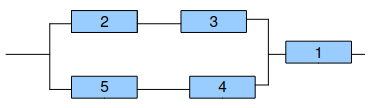
\includegraphics{1.png}
\subsection*{Решение}
Выразим событие
\begin{gather*}
	A_{23} = A_2 \cup A_3 \\
	A_{45} = A_4 \cup A_5 \\
	A_{2345} = A_{23} \cap A_{45} \\
	A = A_{2345} \cup A_1 \\
\end{gather*}
или
\[A = ((A_2 \cup A_3) \cap (A_4 \cup A_5)) \cup A_1\]
Надем вероятность
\begin{gather*}
	P(A_{23}) = 1 - [1 - p_2] \cdot [1 - p_3] \\
	P(A_{45}) = 1 - [1 - p_4] \cdot [1 - p_5] \\
	P(A_{2345}) = P(A_{23}) \cdot P(A_{45}) \\
	P(A) = 1 - [1 - P(A_{2345})] \cdot [1 - p_1]
\end{gather*}
или
\[P(A) = 1 - [1 - \left(1 - [1 - p_2] \cdot [1 - p_3]\right) \cdot \left(1 - [1 - p_4] \cdot [1 - p_5]\right)] \cdot [1 - p_1]\]
Вычислим
\[P(A) \approx 0.7508\]

\newpage

\subsection{Задание \textnumero4.}
Имеется пять урн. В 1-й, 2-й и 3-й урнах находится по 2 белых и 3 черных шара;
в 4 и 5 урнах — по 1 белому и 1 черному.
Случайно выбирается урна и из нее вынимается шар. Он оказался белый.
Какова вероятность того, что выбрана 4-я или 5-я урна?
\subsection*{Решение}
$A$ -- достали белый шар \\
$H_i, i = \overline{1, 5}$ -- достали из $i$-той урны \\
$P(H_i) = \frac{1}{5}, i = \overline{1, 5}$ \\
$P(A|H_1) = P(A|H_2) = P(A|H_3) = \frac{2}{5}$ \\
$P(A|H_4) = P(A|H_5) = \frac{1}{2}$ \\
Применим флрмулу полной вероятности
\begin{gather*}
	P(A) = \sum_{i = 1}^5 P(H_i)P(A|H_i) \\
	P(A) = \frac{11}{25} \\
\end{gather*}
Применим формулу Байеса, чтобы найти $P(H_4|A)$ и $P(H_5|A)$
\begin{gather*}
	P(H_4|A) = \frac{P(H_4)P(A|H_4)}{P(A)} \\
	P(H_4|A) = \frac{\frac{1}{5} \cdot \frac{1}{2}}{\frac{11}{25}} \\
	P(H_4|A) = \frac{5}{22} \\
	P(H_5|A) = \frac{P(H_5)P(A|H_5)}{P(A)} \\
	P(H_5|A) = \frac{\frac{1}{5} \cdot \frac{1}{2}}{\frac{11}{25}} \\
	P(H_5|A) = \frac{5}{22} \\
\end{gather*}
Тогда вероятность того, что выбрана 4-я или 5-я урна:
\begin{gather*}
	P(H_{45}) = P(H_4) + P(H_5) \\
	P(H_{45}) = 2 \cdot \frac{5}{22} \\
	P(H_{45}) = \frac{5}{11} \\
\end{gather*}

\newpage

\subsection{Задание \textnumero5.}
Найти вероятность того, что в серии из 9 подбрасываний игральной кости 5 очков выпадет менее трех раз.
\subsection*{Решение (Бернулли)}
Воспользуемся формулой Бернулли, для определения вероятностей двух событий:
\begin{itemize}
	\item 5 очков выпало ровно один раз \\
	      \begin{gather*}
		      P_n(m) = C_n^mp^mq^{n-m} \\
		      p = \frac{1}{6} \\
		      q = q - p = 1 - \frac{1}{6} = \frac{5}{6} \\
		      P_9(1) = C_9^1p^1q^{9-1} \\
		      P_9(1) = \frac{9!}{(9 - 1)!1!}\frac{1}{6}\left(\frac{5}{6}\right)^8 \\
		      P_9(1) \approx 0.35 \\
	      \end{gather*}
	\item 5 очков выпало ровно два раза \\
	      \begin{gather*}
		      P_9(2) = C_9^2p^2q^{9-2} \\
		      P_9(2) = \frac{9!}{(9 - 2)!2!}\left(\frac{1}{6}\right)^2\left(\frac{5}{6}\right)^7 \\
		      P_9(2) \approx 0.28 \\
	      \end{gather*}
\end{itemize}

Суммараная вероятность:
\begin{gather*}
	P(A) = P_9(1) + P_9(2) \\
	P(A) \approx 0.35 + 0.28 \\
	P(A) \approx 0.63 \\
\end{gather*}

\subsection*{Решение (Пуассона)}
Воспользуемся формулой Пуассона, для определения вероятностей двух событий:
\begin{itemize}
	\item 5 очков выпало ровно один раз \\
	      \begin{gather*}
		      P_n(m) \approx \frac{\lambda^m}{m!}e^{-\lambda}, \lambda = np \\
		      p = \frac{1}{6} \\
		      q = q - p = 1 - \frac{1}{6} = \frac{5}{6} \\
		      P_9(1) \approx \frac{(9 \cdot \frac{1}{6})^1}{1!}e^{-9 \cdot \frac{1}{6}} \\
		      P_9(1) \approx 0.34
	      \end{gather*}
	\item 5 очков выпало ровно два раза \\
	      \begin{gather*}
		      P_9(2) \approx \frac{(9 \cdot \frac{1}{6})^2}{2!}e^{-9 \cdot \frac{1}{6}} \\
		      P_9(2) \approx 0.25
	      \end{gather*}
\end{itemize}

Суммараная вероятность:
\begin{gather*}
	P(A) = P_9(1) + P_9(2) \\
	P(A) \approx 0.34 + 0.25 \\
	P(A) \approx 0.59 \\
\end{gather*}

\subsection*{Решение (Пуассона)}
Воспользуемся формулой Пуассона, для определения вероятностей двух событий:
\begin{itemize}
	\item 5 очков выпало ровно один раз \\
	      \begin{gather*}
		      P_n(m) \approx \frac{\lambda^m}{m!}e^{-\lambda}, \lambda = np \\
		      p = \frac{1}{6} \\
		      q = q - p = 1 - \frac{1}{6} = \frac{5}{6} \\
		      P_9(1) \approx \frac{(9 \cdot \frac{1}{6})^1}{1!}e^{-9 \cdot \frac{1}{6}} \\
		      P_9(1) \approx 0.34
	      \end{gather*}
	\item 5 очков выпало ровно два раза \\
	      \begin{gather*}
		      P_9(2) \approx \frac{(9 \cdot \frac{1}{6})^2}{2!}e^{-9 \cdot \frac{1}{6}} \\
		      P_9(2) \approx 0.25
	      \end{gather*}
\end{itemize}

Суммараная вероятность:
\begin{gather*}
	P(A) = P_9(1) + P_9(2) \\
	P(A) \approx 0.34 + 0.25 \\
	P(A) \approx 0.59 \\
\end{gather*}

\end{document}
